Nello stesso modo con cui abbiamo realizzato la simulazione per lo studio
dell'orbita, lanciamo la simulazione con i parametri settati nel seguente modo
\begin{lstlisting}[language=matlab,breaklines=true]
GravityTypeFlag=1;		%(1=J2 Gravity Model/=0 Spherical)
GravityGradientTorqueFlag=1;	%1=Gravity Gradient Torque ON/0=OFF 
DragForceDisturbancesFlag=1;	%0=Drag Force Disturbance OFF/1=OFF
DragTorquesDisturbancesFlag=1;	%0=Drag Torque Disturbance OFF/1=ON
DragFreeControlFlag=0;		%0=Drag Free Control OFF/1=ON
AttitudeControlFlag=0;		%0=Attitude Control OFF/1=ON
\end{lstlisting}
ovvero, il gradiente di gravità è non sferico, sono presenti le coppie di
disturbo dovute a quest'ultimo e i disturbi dovuti al drag, ma la simulazione
viene eseguita senza azionare alcun controllo.
Di seguito sono i riportati i plot dell'accelerazione dovuta al drag, della
stessa docuta al gradiente di gravità e il plot dell'assetto con i quaternioni.

\begin{SCfigure}[0.7][ht]
	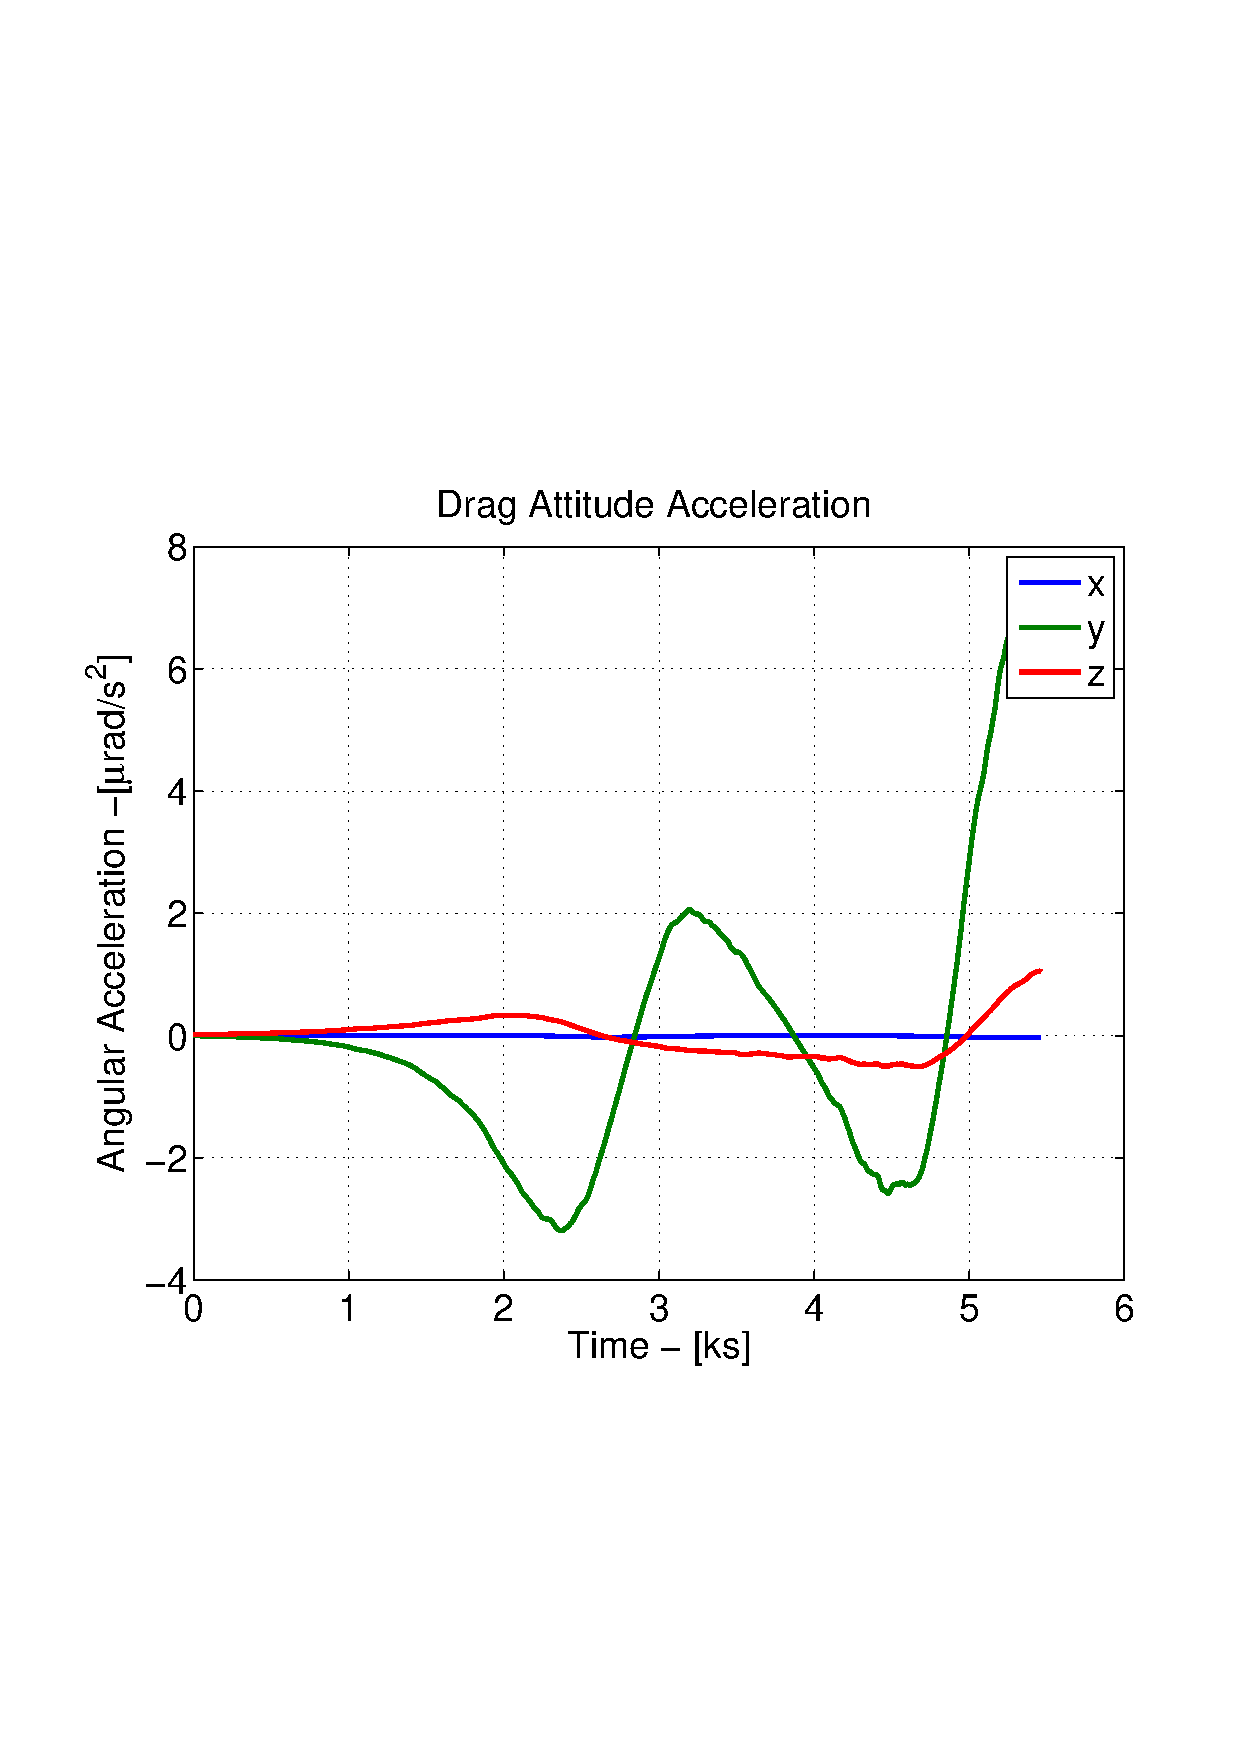
\includegraphics[width=.6\textwidth,clip=true,trim=1cm
	6cm
	1cm
	8cm]{modelling/attitude_kinematics_and_dynamics/image/DragAttitudeAcceleration.pdf}
	\caption{\emph{Accelerazione dovuta al drag} espressa nel riferimento corpo}
	\label{fig:drag-acceleration}
\end{SCfigure}

\begin{SCfigure}[0.7][ht]
	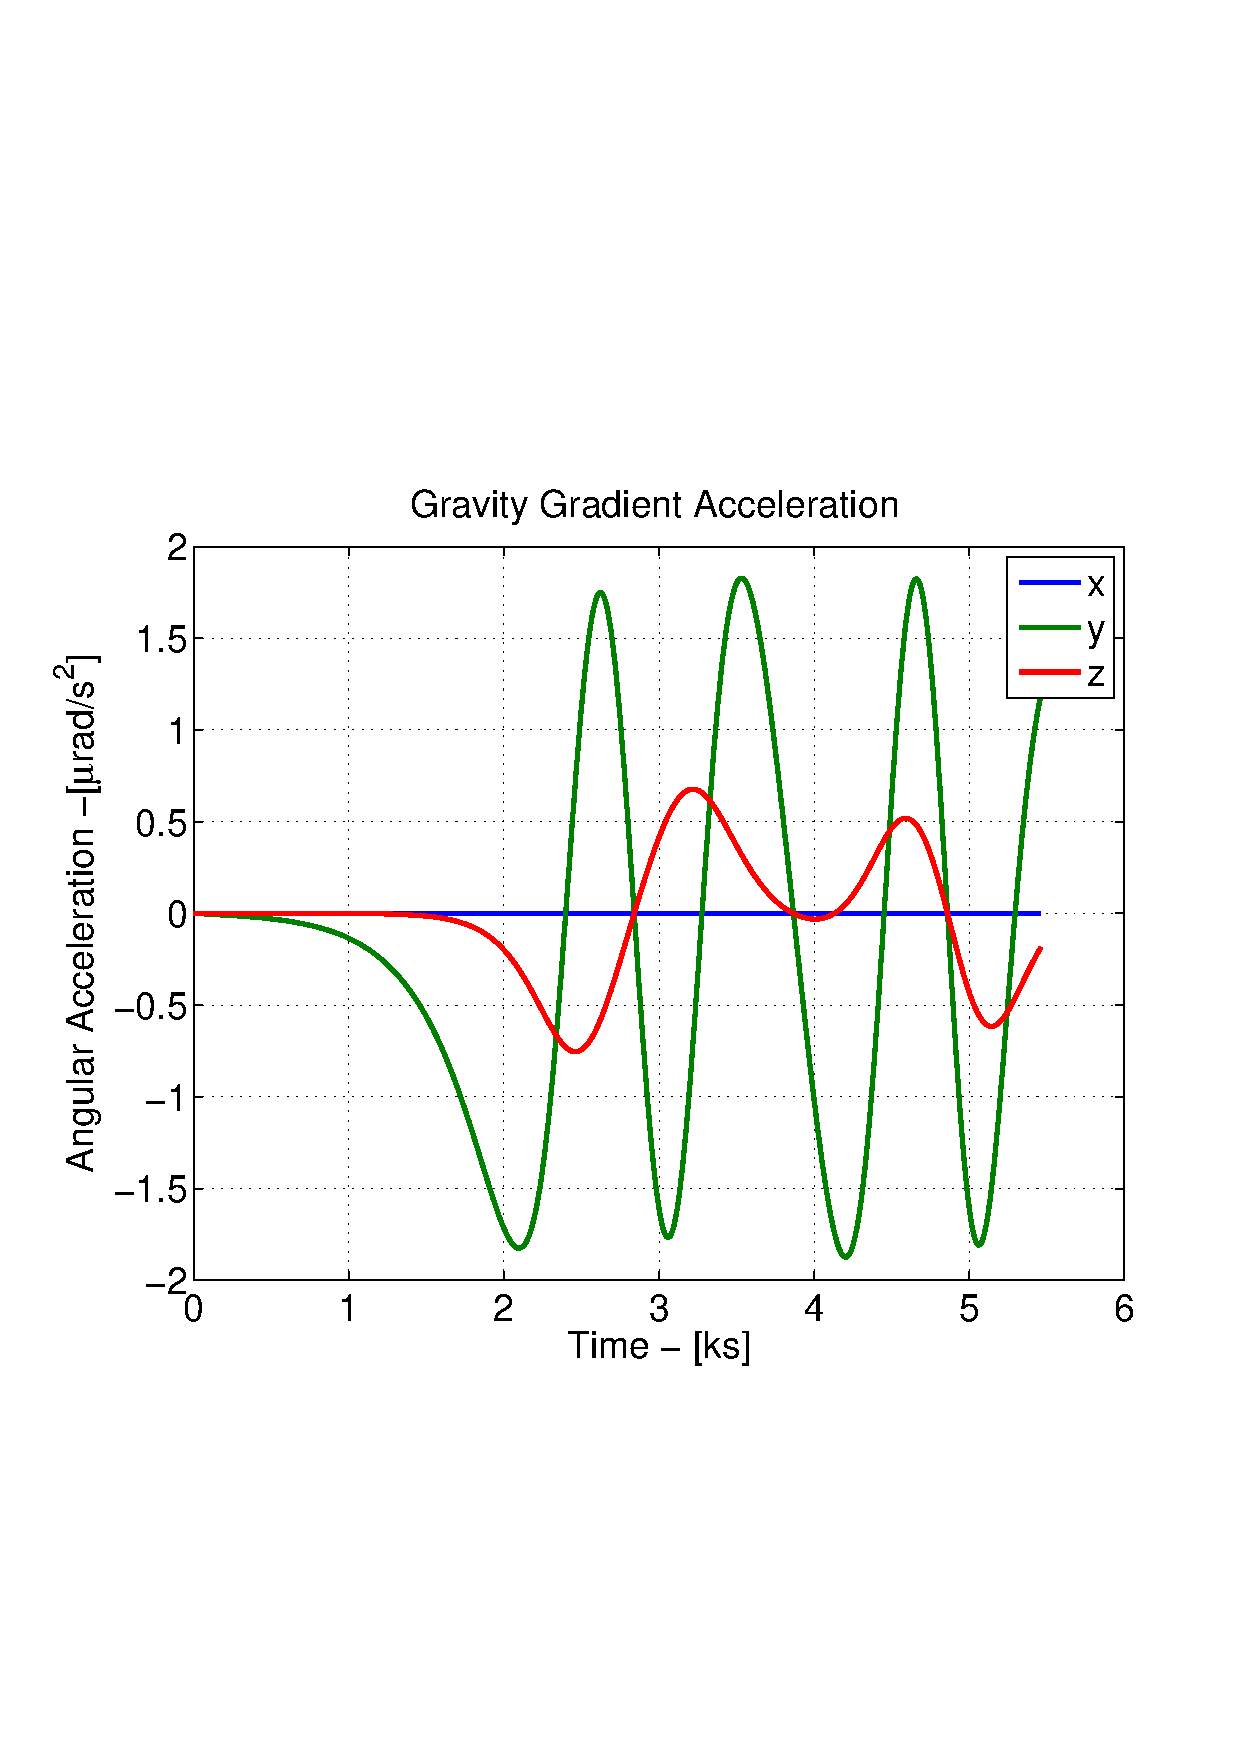
\includegraphics[width=.6\textwidth,clip=true,trim=1cm
	6cm
	1cm
	8cm]{modelling/attitude_kinematics_and_dynamics/image/GravityGradientAcceleration.pdf}
	\caption{\emph{Accelerazione dovuta gradiente di gravità} espressa nel
	riferimento corpo, le variazioni sono dovute all'appiattimento ai poli del
	globo terrestre}
	\label{fig:gravity-acceleration}
\end{SCfigure}

\begin{SCfigure}[0.7][ht]
	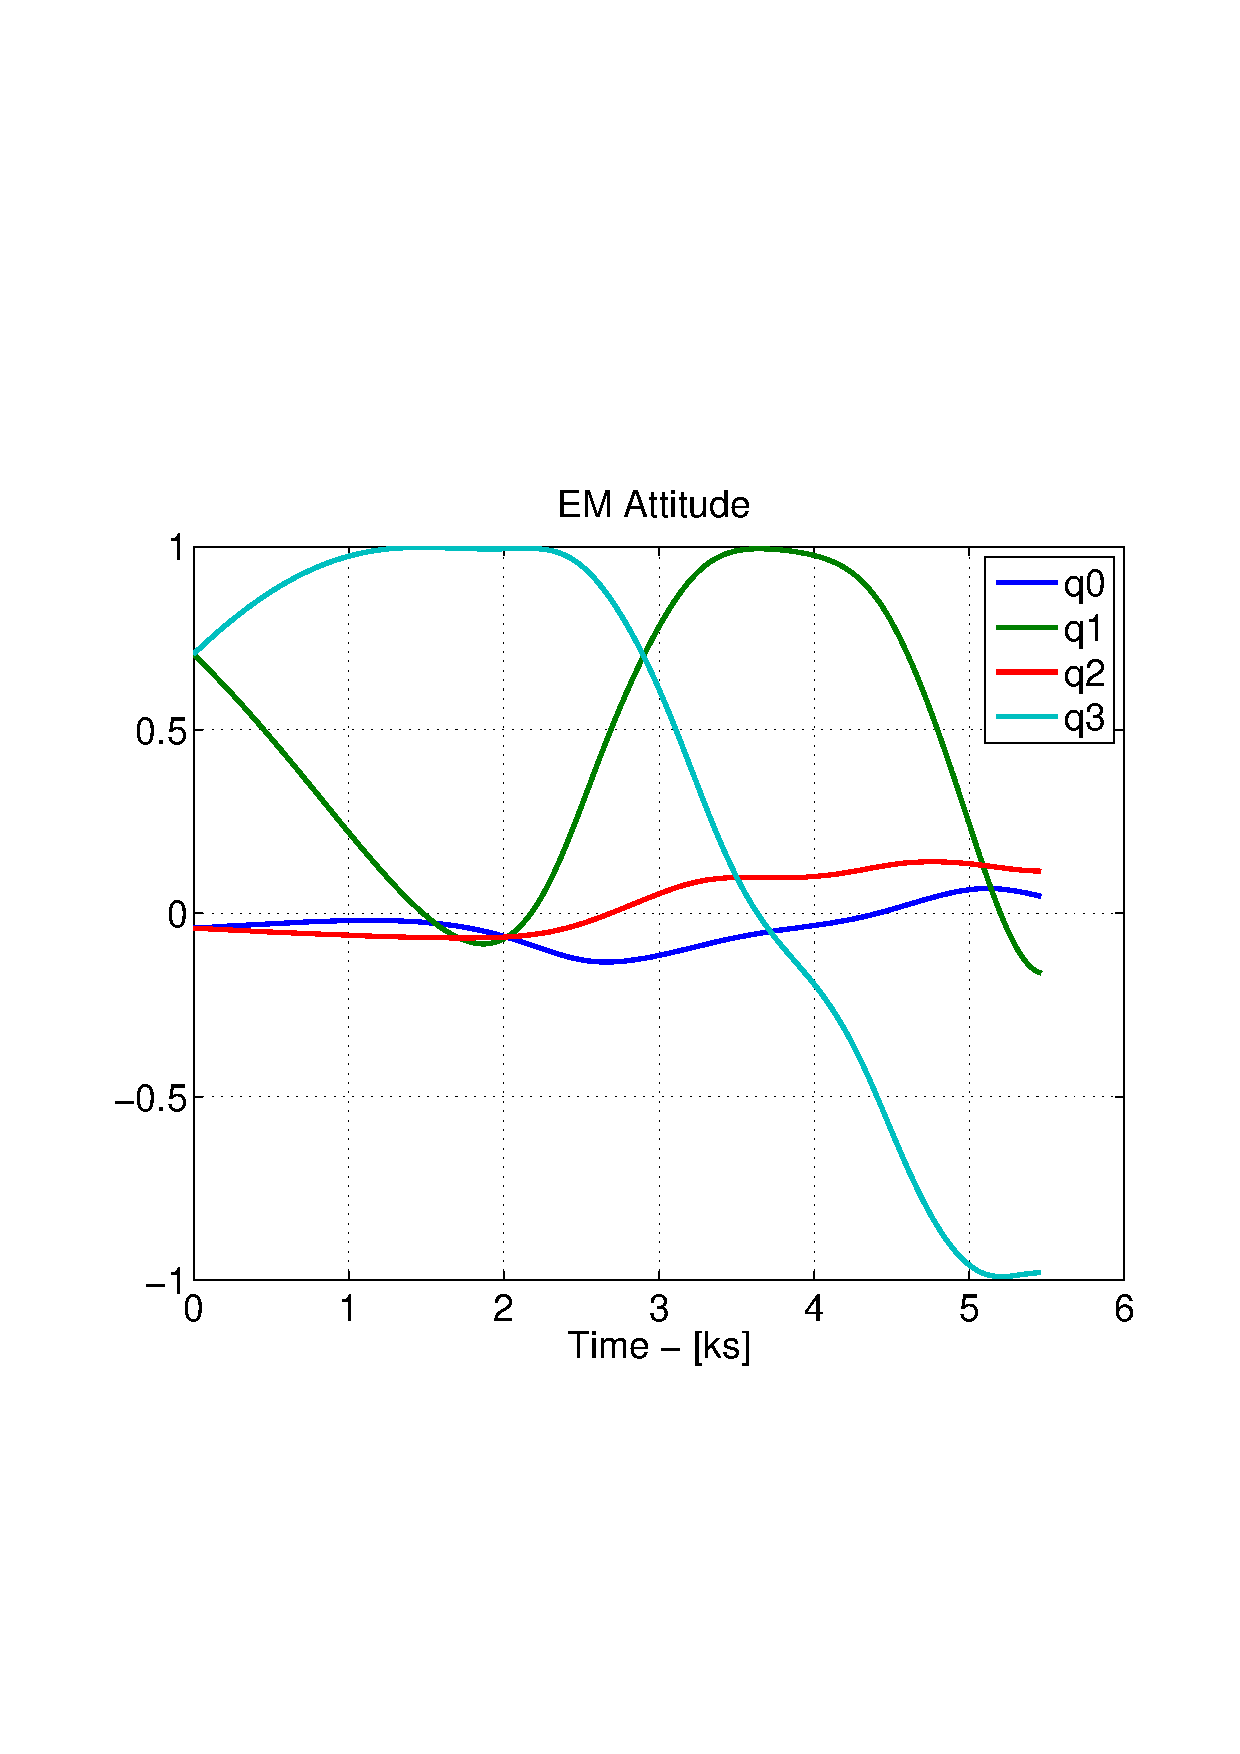
\includegraphics[width=.6\textwidth,clip=true,trim=1cm
	6cm
	1cm
	8cm]{modelling/attitude_kinematics_and_dynamics/image/EMAttitude.pdf}
	\caption{\emph{Assetto} in uscita dall'Embedded Model ed  espresso attraverso
	i quaternioni}
	\label{fig:attitude}
\end{SCfigure}